\chapter{Sensitivity and noise in gravitational wave detectors}
\label{c:instrumentation}

\note{Signal extraction cavity vs signal recycling cavity?}

\section{Interferometer foundations}

The effect that an interferometer has on a means of readout (e.g. a photodetector) as some variable is modulated is termed the \emph{response}. The most important response to consider in gravitational wave interferometry is the arm cavity differential degree of freedom's response to the beam splitter's output port. The response varies as a function of frequency depending on the interferometer topology and its light storage time. For instance, in a Michelson interferometer the dARM response is typically flat for frequencies below the arm cavity pole, and decaying \checkme{at a rate proportional to frequency} above. At higher frequencies, less light can be stored as the cavity cannot build up sufficient light power due to mirror loss and round-trip time. This effect is shown in \note{Figure XXX} for different end test mass reflectivities and in \note{Figure XXX} for different arm cavity lengths.

In order to calculate a response function for a set of optics, it is necessary to understand the propagation of a light field through vacuum and through optics.

\note{Reference the appendix on interferometry fields etc.}

\note{Describe use of laser frequency to measure length}
\begin{equation}
  \label{eq:freq-to-length}
  \frac{\Delta f}{f} = \frac{\Delta L}{L}
\end{equation}


\subsection{\label{sec:operating-point}Operating point}
In precision measurement, typically an experimentalist can only infer the quantity of an underlying amplitude from a measured power. A simple example is the measurement of mirror displacement in a simple Michelson interferometer \emph{via} the photocurrent output of the photodetector. The wave is composed of the electric and magnetic fields, $E$ and $B$, respectively, each of which can be expressed as a travelling wave:
\begin{align}
  E &= E_0 \text{e}^{\text{i} \left( kx - \omega t \right)}, \\
  B &= B_0 \text{e}^{\text{i}  \left( kx - \omega t \right)},
\end{align}
where $E_0$ and $B_0$ are the initial field amplitudes, $k = \frac{2 \pi}{\lambda}$ is the wave vector, $x$ is the displacement, $\omega$ is the angular frequency and $t$ is time. The intensity $S$ is the product of the two, with the magnetic field weighted by the permittivity of free space $\epsilon_0$ and speed of light in vacuum $c_0$ \checkme{check this is consistent with Living Review p31}:
\begin{equation}
  S = \frac{1}{2} \epsilon_0 \left( E^2 + c_0^2 B^2 \right).
\end{equation}
As the $E$ and $B$ fields are orthogonal, their sum at any point in time and space remains constant. We can therefore state that the wave's intensity is proportional to the square of an ``amplitude'' $A$, expressing the combination of $E$ and $B$:
\begin{equation}
  S \propto A^2.
\end{equation}
Leaving the beam splitter towards the end of each arm, each wave in the Michelson interferometer propagates with amplitude
\begin{equation}
  A = A_{\text{in}} \text{e}^{\text{i} \left( kx - \omega t \right)},
\end{equation}
where $A_{\text{in}}$ represents the field at the beam splitter's input.

A difference in path length between the arms $\Delta x$ leads to a difference in round-trip phase between light returning to the beam splitter. With light of constant amplitude injected into the interferometer, and assuming that the light round-trip time is much quicker than the transient causing a change to the arm lengths, we can look at the superposition of returning light at the beam splitter to determine the change in path length. At the beam splitter's output port, the field superposition becomes:
\begin{equation}
  A_{\text{out}} = \frac{A_{\text{in}}}{2} \text{e}^{\text{i} \left( k \left( x + \frac{\Delta x}{2} \right) - \omega t \right)} + \frac{A_{\text{in}}}{2} \text{e}^{\text{i} \left( k \left( x - \frac{\Delta x}{2} \right) - \omega t \right)},
\end{equation}
where we assume that the path length difference caused by the transient is evenly distributed, differentially, between the two arms. The power measured by a photodetector, $P_{\text{out}}$, is then the field multiplied by its complex conjugate:
\begin{equation}
  \label{eq:mich-p-out}
  \begin{split}
    P_{\text{out}} &\propto \langle A_{\text{out}}^*A_{\text{out}} \rangle \\
                   &= \frac{P_{\text{in}}}{2} \left( 1 + \cos \left( k \Delta x \right) \right),
  \end{split}
\end{equation}
using the fact that $P_{\text{in}} = A_{\text{in}}^2$. This shows that the signal from the arm length motion is encoded in the phase of the signal witnessed by the photodetector at the output port.

Getting access to the phase information encoded within the light is more difficult than making a simple measurement of power. Sections \note{WGM PDH, controls BHD and ET DC readout} describe techniques to access this information given different noise and signal constraints.

\note{Explain dark fringe offset}

\subsection{Numerical simulation tools}
Recall the reflection term $r$ we ignored earlier. Light propagating within an interferometer will collect reflection and transmission terms from each mirror it encounters. A photodetector placed at a port of the interferometer will then see light with amplitude and phase information representing the path it has taken through the interferometer. We have shown this effect in a trivial example involving a \FP{} cavity with one input, but the same mathematics can be used to represent any interferometer. For anything beyond the simplest of examples, we typically employ numerical simulation tools to perform the tedious calculations involved in obtaining the output signals from interferometers, with the packages Finesse \cite{Freise2004} (not to be confused with \emph{cavity} finesse) and Optickle \cite{Evans2012} being popular choices within the field of gravitational wave interferometry.

\section{\label{sec:ifo-noise}Measurement noise in gravitational wave interferometry}
Measurement precision is ultimately a matter of \emph{signals} and \emph{noise}. The term ``signal'' simply refers to a wanted pattern of oscillations representing a particular variable of interest. ``Noise'', on the other hand, is unwanted oscillations that appear at the signal measurement device. In reality the measurement of any signal necessarily entails the measurement of some noise.

Gravitational wave observatories are limited by a plethora of noise sources both fundamental and technical. In order to understand how to mitigate sources of noise in interferometers, it is necessary to understand how they arise and utilise techniques to mitigate them. The initial generation of detectors was limited by a range of different noise sources, and the knowledge gained from the first science runs fed in to the design of the second generation of detectors.

The creation of \emph{noise budgets} from theoretical descriptions of sources is a useful way to examine how they influence the sensitivity of an experiment. The noise budget for \ALIGO{} is shown in Figure\,\ref{fig:aligo-noise-budget}. At its most sensitive frequencies, \ALIGO{} is limited by quantum and thermal noise, whilst at lower frequencies the motion of the ground from seismic sources sets the limit. Careful design involving specially selected materials and techniques has reduced thermal noise arising from the mirror coatings and suspensions and technical noise associated with electronics and facilities. Quantum noise sets the fundamental limit given the available light power and mirror masses utilised in \ALIGO{} and \AVIRGO{}, and in order to improve the sensitivity beyond the limit set by quantum noise, approaches that involve changing the nature of the quantum interactions within the interferometer have to be implemented. Individual noise sources are discussed throughout the rest of this chapter.

\begin{figure}
  \centering
  \includegraphics[width=\columnwidth]{graphics/generated/from-python/20-aligo-noise-budget.pdf}
  \caption[Advanced LIGO noise budget]{\label{fig:aligo-noise-budget}Advanced LIGO noise budget. Greater sensitivity to gravitational waves is achieved by having lower residual strain noise. The strain noise limit is shown in \checkme{black}, which is the incoherent sum of the noise sources from other effects. All of the noise sources shown have some frequency dependence, and optimal sensitivity in a detector is reached by designing the experiment in such a way as to minimise the noise sources in the frequency band of interest. The creation of budgets like this from theoretical descriptions of noise sources is a useful way in which to understand how they affect the sensitivity.}
\end{figure}

\subsection{\label{sec:noise-via-loss}Noise arising from loss and uncertainty}
Quantum mechanics shows that the universe contains a continuous spectrum of quantum fluctuations at all frequencies. Virtual photons are constantly being created and annihilated everywhere, albeit with an average energy of zero, producing the measurement uncertainty required by quantum laws. An interferometer's cavities create local filters of this quantum spectrum which allow a certain subset of vacuum modes to circulate. Virtual photons are able to enter the interferometer via its loss points, just as virtual photons created within the interferometer are allowed to leave. In this way, non-unity reflectivity of optics, scattering and other photon loss effects within an interferometer lead to the intrusion of vacuum noise.

In lasers, a pumped electromagnetic field creates a coherent state which can be propagated through an interferometer to pick up phase shift due to passing gravitational waves. This typically involves pumping the field into the \emph{coherent} state, in which the average laser amplitude is well defined, and noise arises from the presence of virtual photons in the pumped field leading to an uncertainty in the number of photons output from the laser.

In materials, phonons \checkme{arising from thermal energy uncertainty} have a similar effect to vacuum fluctuations and lead to thermal noise.

In general, the noise arising from fluctuations is quantified by the fluctuation dissipation theorem developed in the early \nth{20} Century, which shows that the noise spectral density due to fluctuations:
\begin{equation}
  S_{\text{fluc}} \propto \frac{T}{Q},
\end{equation}
is related not only to the temperature $T$, but also to the quality factor $Q$ relating to the loss of the material. Other examples of noise from fluctuations are, for example:
\begin{itemize}
  \item Brownian motion in fluids, where the position of particles suspended in fluid is randomly perturbed due to thermal fluctuations of the molecules forming the liquid;
  \item black body radiation, arising from thermal fluctuation of electrons in matter leading to the production of electromagnetic radiation;
  \item and Johnson-Nyquist noise caused by the creation of noise voltage due to thermal fluctuation of electrons in resistors.
\end{itemize}

The effect of noise on the interferometer can be calculated by quantifying the magnitude of noise entering at the loss point and propagating this noise as if it were signal to the sensor. The noise at a photodetector is therefore the sum of noise propagated from each point of loss. The way in which some forms of noise enters a \DRFPMI{} and propagates to the output port is shown in Figure\,\ref{fig:modelling-noise}.

\begin{figure}
  \centering
  \includegraphics[width=\columnwidth]{graphics/generated/from-svg/20-modelling-noise.pdf}
  \caption[Modelling noise]{\label{fig:modelling-noise}Blah}
\end{figure}

\subsection{Thermal noise}
Thermal noise arises from loss in materials used to reflect and focus light and to suspend test masses, where photons in the thermal state are allowed to enter the interferometer and propagate to the sensors.

Thermal noise arises from a material's \emph{loss angle}, which is the imaginary part of the Young's modulus, relating applied stress to the strain of the material. The material with a high loss angle results in an applied stress creating an associated strain at a different time, and during this time the wave can accumulate noise via thermal fluctuations of the material. Thermal noise in gravitational wave detectors arises mainly from the test mass optical coatings and suspensions.

\subsubsection{\label{sec:coating-thermal-noise}Coating thermal noise}
In the conceptual design for the first generation of gravitational wave detectors such as GEO-600 \cite{Willke2002} the designers were not aware that thermal noise associated with the reflective coatings on mirrors would play a significant role in the sensitivity of the interferometers. For a long time it was known that thermal noise would contribute to the sensitivity of the detectors, particularly from the bulk material forming the test masses, but it soon became clear as the detectors were being commissioned that thermal noise arising from the reflective mirror coatings would dominate the thermal noise associated with the test masses in the frequency band of interest despite forming only a tiny fraction of the test masses by volume. Investigations conducted by Harry \etal{} \cite{Harry2002, Harry2007}, among others, concluded that mechanical loss present in the dielectric coatings on the test masses led to Brownian noise creating a limit to the sensitivity of detectors across a wide range of frequencies. Contributions from thermoelastic noise, arising from the thermal expansion coefficient of the materials of the coatings \cite{Braginsky1999a}, and thermorefractive noise, arising from the change in refractive index caused by such expansion \cite{Braginsky2000a}, produce further noise contributions which will become more important as coatings with improved thermal noise contributions are developed.

Over the past two decades, efforts have been made to both quantify and reduce coating thermal noise. Particular interest is being paid to the study of coatings for cryogenically cooled mirrors, such as the sapphire (\ce{Al_2O_3}) test masses to be used in the Japanese detector \gls{KAGRA} \cite{Somiya2012}. A loss peak in the mirror material silica, for detectors until recently ubiquitous, occurs at low temperature. This makes the material unsuitable for cryogenic use, as mechanical loss will couple into the light within the interferometer and make its way to the detection port. Other materials such as sapphire do not feature this loss peak and provide lower thermal noise than silica at room temperature for a given mirror design. Coating noise is also proportional to temperature, so cryogenically cooled mirrors can offer better performance. Additionally, crystalline coatings made from compounds such as \ce{AlGaAs} can offer future detectors a coating thermal noise reduction of up to 3 over current state of the art \cite{Cole2013} if technical challenges in their manufacturing can be overcome.

The dominant contribution to coating noise in gravitational wave detectors comes from Brownian noise, given as \cite{Harry2002}:
\begin{equation}
  S_{\text{x, coating}} = \frac{2 k_B T}{\pi^{3/2} f} \frac{1}{w Y} \left( \phi_{\text{sub}} + \frac{1}{\sqrt{\pi}} \frac{d}{w} \left( \frac{Y'}{Y} \phi_{\text{para}} + \frac{Y}{Y'} \phi_{\text{perp}} \right) \right),
\end{equation}
with $k_B$ Boltzmann's constant, temperature $T$, frequency $f$, beam size $w$, Young's moduli $Y$, loss angle $\phi$ and coating thickness $d$. The Young's moduli and loss angles are split into components representing the substrate and coatings, and the measurement and interaction between these components is an active area of research. Figure\,\ref{fig:aligo-noise-budget} shows coating Brownian noise jointly dominating the noise at frequencies around \SI{70}{\hertz}.

A mirror topology which avoids the use of many alternating coating layers can potentially offer an improvement in noise performance. Mirrors employing grating structures can resonantly reflect light with less coating material than similarly performing dielectric mirrors \cite{Mashev1985}, though at the expense of additional technical complexity in their utility in gravitational wave detectors \cite{Leavey2015}. Chapter\,\ref{c:waveguides} discusses a form of grating mirror for use in interferometers.

\subsubsection{\label{sec:sus-thermal-noise}Suspension thermal noise}
The test masses in audio-band gravitational wave detectors are suspended from pendulum systems, and current generation observatories (with the notable exception of \KAGRA{}) all utilise fused silica (\ce{SiO2}) fibres, a technique pioneered in \GEO{}. The reason for the use of this material is that the thermal noise present within the metal steel loops used previously was high enough to impart significant motion to the test mass in the gravitational wave channel, with the noise becoming dominant at frequencies around \SI{100}{\hertz} where the interferometer would otherwise be most sensitive \cite{Hammond2012}. Due to its high quality factor, fused silica has reduced mechanical loss and therefore lower noise. Figure\,\ref{fig:aligo-noise-budget} shows that suspension thermal noise is no longer a dominant noise source, unlike in \ILIGO{} \note{make sure initial ligo is defined somewhere}.

As \KAGRA{} will be a cryogenic detector, it does not gain the same noise benefit from using fused silica. Instead, it will use crystalline sapphire which offers similar noise performance at low temperatures.

At higher frequencies, suspension \emph{violin modes} have a significant influence on the measured noise \cite{Robertson2002}. A violin mode with high quality factor can resonantly enhance noise such that it dominates all other sources in a narrow band at frequencies starting around \SI{1}{\kilo\hertz}\footnote{Figure\,\ref{fig:aligo-noise-budget} appears to show that violin modes are not dominant, however the narrow linewidth of the noise is such that the resolution is insufficient to show the effect.}. This is reduced through the use of heavier test masses, which push the violin mode frequencies higher, away from the detection band, and via the use of special monitoring and damping techniques \cite{Sorazu2010} \note{reference to Advanced LIGO controls paper or document regarding damping of modes?}.

\subsection{Quantum noise}
% previously from chapter 4
Arising from the Heisenberg Uncertainty Principle, the quantum noise present within a classical interferometer\footnote{Note the misnomer: a \emph{classical} interferometer can still be limited by \emph{quantum} noise. The name refers to the readout technique, namely the measurement of classical light power to determine displacement.} limits its sensitivity.

One of the results of quantum theory is that two non-commuting observables cannot be simultaneously known to full precision. For two operators $\hat{O}_+$ and $\hat{O}_-$, there exists an error $\epsilon$:
\begin{equation}
 \left[ \hat{O}_+, \hat{O}_- \right] = \epsilon,
\end{equation}
and this means that the observables contain correlated components and as such cannot be considered entirely separate entities. Measuring one observable automatically influences the other, leading to the well-known \emph{Heisenberg Uncertainty Principle}:
\begin{equation}
 \left| \Delta \hat{O}_+ \right| \cdot \left| \Delta \hat{O}_- \right| \geq
\frac{1}{2} \left| \epsilon \right|,
\end{equation}
where $\Delta$ represents the uncertainty in the given operator, in this case defined as the standard deviation.

\subsubsection{\label{sec:operator-uncertainty}Position, momentum, phase and photon number uncertainty}

In the field of gravitational wave interferometry there are two pairs of operators of particular importance, namely the position and momentum operators, $x$ and $p_x$, and the photon number and phase operators, $n$ and $\phi$, respectively. The canonical commutation relation between $x$ and $p_x$ is given as:
\begin{equation}
 | \Delta x\left( t \right) | \cdot |\Delta p\left( t \right) | \geq
\frac{\hbar}{2},
 \label{eq:heisenburguncertainty}
\end{equation}
where $\hbar$ is the reduced Planck constant. Consider a position measurement of a free mirror of mass $m$ being perturbed by a signal of frequency $f$. If a measurement is made at time $t$ and then again at time $t + \Delta t$, the uncertainty on the latter can be expressed in terms of the uncertainty in momentum of the mirror multiplied by the time difference:
\begin{equation}
 \Delta x \left( t + \Delta t \right) = \Delta x \left( t \right) + \Delta p_x
\left( t \right) \frac{\Delta t}{m}.
 \label{eq:heisenburgtime}
\end{equation}
This result shows that the momentum of the mirror at time $t$ influences the position of the mirror at a later time. Since momentum is position scaled by velocity, this leads to a minimum value on which $x \left( t \right)$ can take:
\begin{equation}
 \Delta x \left( t \right) \geq \sqrt{\frac{\hbar \Delta t}{2m}}.
\end{equation}
The key result to highlight here is that, even with an otherwise unperturbed mirror, the momentum imparted by the measurement at time $t$ influences the later measurement at $t + \Delta t$ in such a way that it adds uncertainty. Or, put another way, Equation\,\ref{eq:heisenburguncertainty} expresses that the smaller the error on the position of an observable in a quantum mechanical system, the greater the error on the momentum; and vice-versa.

We typically make position measurements indirectly via the change in phase of photons from a laser. In this case, the most appropriate uncertainty relation to use is the photon number-phase relation:
\begin{equation}
  \label{eq:photon-phase-hup}
  \Delta n \Delta \phi \geq \frac{1}{2}.
\end{equation}
Assuming that a photodetector has incident upon it $n$ photons in a given interval, the standard deviation of the number of photons detected per unit time will follow Poisson statistics, i.e. $\Delta n = \sqrt{\bar{n}}$, where $\bar{n}$ is the average photon number calculated by considering many intervals. A single photon has energy $E_P$ given by the standard relation involving frequency $f$:
\begin{equation}
  E_P = hf,
\end{equation}
and so the power in the beam at a given interval is then:
\begin{equation}
  \begin{split}
    P &= E_P n \\
      &= hfn.
  \end{split}
\end{equation}
The measurement of power is simply the energy multiplied by its complex conjugate, i.e. $P = E^{\ast}E$, and so we can recover the original energy of the light from the measurement of power:
\begin{equation}
  \left| E \right| = \sqrt{hfn}.
\end{equation}
Given that:
\begin{equation}
  \frac{\Delta \left| E \right|}{\Delta n} = \frac{d \left| E \right|}{dn},
\end{equation}
we can obtain the standard deviation of the measured amplitude:
\begin{equation}
  \label{eq:std-dev-amp}
  \begin{split}
    \Delta \left| E \right| &= \frac{d \left| E \right|}{dn} \Delta n \\
                            &= \frac{1}{2} \sqrt{\frac{hf}{n}} \Delta n \\
                            &= \frac{1}{2} \sqrt{hf} \\
                            &= \frac{1}{2} \sqrt{E_P}.
  \end{split}
\end{equation}
Note that this variation does not depend on photon number, and is instead defined only in terms of a fundamental constant and the laser frequency. This is the origin of quantum noise, and the lack of light power dependence justifies the inclusion of arm cavities in gravitational wave detectors as discussed in Section\,\ref{sec:fabry-perot-cavities}.

The effect the amplitude variation has on the phase uncertainty can be calculated by expressing it as the fractional energy uncertainty:
\begin{equation}
  \label{eq:phase-uncertainty}
  \begin{split}
    \Delta \phi &= \frac{\Delta \left| E \right|}{\left| \bar{E} \right|} \\
                &= \frac{\sqrt{hf}}{2} \frac{1}{\sqrt{hf \bar{n}}} \\
                &= \frac{1}{2 \sqrt{\bar{n}}} \\
                &= \frac{1}{2 \Delta n}.
  \end{split}
\end{equation}
From the last line in Equation\,\ref{eq:phase-uncertainty} we can recover a result resembling that given in Equation\,\ref{eq:photon-phase-hup}:
\begin{equation}
  \label{eq:photon-phase-hup-min}
  \Delta n \Delta \phi = \frac{1}{2}.
\end{equation}
The reason for the $=$ in Equation\,\ref{eq:photon-phase-hup-min} is that an assumption has been made in Equation\,\ref{eq:std-dev-amp} that the energy uncertainty is made from equal parts amplitude and phase uncertainty. This is called a \emph{coherent state} and this approximates what a standard laser will output\footnote{Actually, lasers are typically quite incoherent on their own, and experimentalists must first ``mode clean'' the light to remove unwanted incoherent states. Special mode-cleaning cavities are implemented in most experiments to perform this task.}. Equation\,\ref{eq:photon-phase-hup} contains a $\geq$ and is therefore a general equation representing all states, including \emph{squeezed} states, which will be discussed in Section\,\ref{sec:squeezing}.

\subsubsection{Quantum shot noise}
As described in Section\,\ref{sec:noise-via-loss}, open ports in the interferometer allow vacuum noise to enter. When this noise is measured by a photodetector it is termed \emph{quantum shot noise}, and it arises directly from the phase uncertainty derived in Section\,\ref{sec:operator-uncertainty}. We change representation from discrete pulses to a continuous measurement made by a laser by representing $n$ in Equation\,\ref{eq:photon-phase-hup-min} as a light power $P$ via the relation $n = \frac{P \Delta t}{\hbar \omega_0}$, where $\omega_0$ is the laser's angular frequency. The displacement-equivalent shot noise power spectral density then arises from the phase uncertainty:
\begin{equation}
  \label{eq:shot-noise-psd}
  S_{\text{shot}} = \frac{\hbar c^2}{P \omega_0}.
\end{equation}
As quantum noise arises from vacuum noise\textemdash spontaneous creation and annihilation of photons in the vacuum\textemdash it is a statistical random process and so the shot noise spectral density in Equation\,\ref{eq:shot-noise-psd} has equal power at all frequencies (it is \emph{white} noise).

The detrimental effect of counting statistics due to phase uncertainty is mitigated by an increase in the classical light power within the interferometer. As the noise entering the interferometer is a function of loss and is, to first order, not dependent upon laser power, higher input light power leads to an increase in signal with respect to noise and so the effect that the noise has on the output is diminished.

\subsubsection{Quantum radiation pressure noise}
Despite being massless, photons impart momentum to mirrors upon reflection proportional to their wavelength. The strongest effect this has on an interferometer is in the \emph{\gls{DC} radiation pressure} effect, which arises from the classical light power circulating within the interferometer. In a classical interferometer this radiation pressure effect expands the arm cavity length \checkme{proportionally to the light power}, with the equilibrium point being defined by the equivalence of the radiation pressure force to the mirror's restoring force.

\emph{Quantum} radiation pressure, on the other hand, arises from the momentum imparted onto mirrors within the interferometer by virtual photons present within the interferometer from the laser and loss points, as shown in Section\,\ref{sec:noise-via-loss}. As with quantum shot noise this effect is related to the input power of the interferometer, $P$, but this time the input power facilitates the phase fluctuations that become transformed into displacement noise via the dynamics of the mirror. The mirror dynamics govern the displacement noise due to back-action. The spectrum of noise from virtual photons is white, and so the energy imparted to the mirror is the same at all frequencies and therefore the effect of radiation pressure follows an inverse frequency relation.

The radiation pressure noise power spectral density is given as \cite{Danilishin2012}:
\begin{equation}
  \label{eq:rp-noise-psd}
  S_{\text{rp}} = \frac{\hbar P \omega_0}{c^2 m^2 \omega^4},
\end{equation}
with reduced mirror mass $m$ and angular frequency of oscillation $\omega = 2 \pi f$. The displacement spectral density, which is $\sqrt{S_{\text{rp}}}$, shows the noise is proportional to $\frac{1}{f^2}$ as expected from a free mass.

\subsubsection{\label{sec:sql}The Standard Quantum Limit}
Note that Equation\,\ref{eq:rp-noise-psd} is proportional to power whilst Equation\,\ref{eq:shot-noise-psd} is inversely proportional to power. This creates a lower bound on the sensitivity of a classical interferometer though a manifestation of the Heisenberg Uncertainty Principle, termed the \emph{standard quantum limit} (\gls{SQL}).

The \gls{SQL} is the point at which the quadrature sum of shot and radiation pressure noise is minimised, and this occurs when the individual components are equal. For each laser power there exists a single frequency at which the \gls{SQL} can be reached. The \gls{SQL} forms a sensitivity limit proportional to $\frac{1}{f^2}$ which can only be crossed with special, \emph{sub}-\gls{SQL} techniques. In terms of strain, the \gls{SQL} is defined for a \MI{} as \cite{Braginsky1996}:
\begin{equation}
  \label{eq:strainsql}
  h_{SQL} = \sqrt{\frac{8 \hbar}{m \Omega^2 L^2}},
\end{equation}
where $L$ represents the \MI{}'s arm length.

The spectrum of a \MI{} is defined as:
\begin{equation}
  \label{eq:classicalifospectrum}
  S_h = \frac{h^{2}_{SQL}}{2} \left( \frac{1}{\kappa} + \kappa \right),
\end{equation}
where the \gls{SQL} is reached only at a single frequency. The term $\kappa$ is defined as the \emph{opto-mechanical coupling constant}:
\begin{equation}
 \kappa = \frac{I_0}{I_{SQL}} \frac{2 \gamma^4}{\Omega^2 \left( \gamma^2 +
\Omega^2 \right)},
 \label{eq:optomechanicalcoupling}
\end{equation}
with $I_0$ the laser power at the beam splitter, $I_{SQL}$ the laser power required to reach the \gls{SQL}, $\gamma$ the cavity half-bandwidth, and $\Omega$ the gravitational wave frequency. $I_{SQL}$ can be itself defined as:
\begin{equation}
 I_{SQL} = \frac{m L^2 \gamma^4}{4 \omega_0},
\end{equation}
with $m$ the mirror mass, $L$ the arm length and $\omega_0$ the light's angular frequency.

The \gls{SQL} is defined at all frequencies, while the spectral density of a quantum noise limited interferometer touches the \gls{SQL} at only one frequency, defined by the mirror mass, light power, arm length and cavity bandwidth. By making a more precise measurement, i.e. one involving more photons carrying information of the mirror motion, we see a smaller shot noise spectral density (we reduce $\Delta n$) whilst we see a larger radiation pressure noise spectral density (we increase $\Delta \phi$) \cite{Caves1981}. This situation is illustrated in Figure\,\ref{fig:sql-vs-input-power} for different input powers.

\begin{figure}
  \centering
  \includegraphics[width=\columnwidth]{graphics/generated/from-python/20-sql-vs-power.pdf}
  \caption[Standard quantum limit and the quantum noise with various input powers]{\label{fig:sql-vs-input-power}The \gls{SQL} for a Michelson interferometer with arms of length \SI{1}{\kilo\meter}, mirrors with reduced mass \SI{50}{\kilo\gram} and optimal frequency \SI{100}{\hertz}, along with quantum noise limited sensitivity curves for three different input powers. The higher the input power, the higher the strain sensitivity can be pushed, but at the expense of higher radiation pressure noise and thus higher optimal frequency for a given interferometer configuration. Quantum non-demolition techniques can be used to surpass the \gls{SQL} (see Section\,\ref{sec:sub-sql-techniques}).}
\end{figure}

An important distinction to make here is that the \gls{SQL} is defined for \emph{uncorrelated} shot and radiation pressure noise. Techniques exist in theory and practice to reduce overall noise by producing correlations between the two effects with so-called \emph{quantum non-demolition} interferometry. \note{See sections...}

\subsection{Other fundamental noise}

\subsubsection{\label{sec:seismic-noise}Seismic noise}
The Earth's surface vibrates with a large amplitude and slow frequency \cite{ET2011}. At around \SI{10}{\micro\hertz} tidal forces due to the gravitational interaction between the Earth and Moon dominate the spectrum, producing displacements of up to \SI{100}{\micro\meter} \cite{Adhikari2004}. At around \SI{0.15}{\hertz} the swell of the ocean can be measured almost anywhere on the Earth, even far from coasts. These effects combine to produce a large amount of seismic noise at low frequencies which must be filtered. As this noise is large in amplitude, it is able to move test masses in laser cavities far enough that they no longer fulfil the resonant condition and lose light power. In almost all audio-band interferometric experiments a large degree of isolation must be utilised to mitigate seismic noise. In Advanced \gls{LIGO}, active platforms are used to damp this motion, sitting atop passive damping materials. The test masses are suspended from many pendulum stages to isolate higher frequencies such that by \SI{10}{\hertz} the ground motion is suppressed by \checkme{10 orders of magnitude}.

\subsubsection{Gravity-gradient noise}
Changes in the density of the ground near the test masses created by seismic noise can couple to the gravitational wave channel via \emph{gravity-gradient} noise, also referred to as \emph{Newtonian} noise. Few experiments have successfully been able to decouple this subtle effect from other sources of noise, but it is believed from extensive modelling effort that this noise source will represent a problem particularly for low frequency detectors such as \ETLF{} \cite{ET2011, Hild2011}. Simulations have shown a benefit in locally shaping the profile of the ground near test masses \cite{Harms2014}, potentially creating a benefit for future ground-based detectors, as well as through the subtraction of gravity-gradient noise inferred from a series of auxiliary witness sensors \cite{Harms2015}.

\subsection{Technical noise}

\subsubsection{Laser frequency and intensity noise}
A perfect laser provides output at a single, well defined frequency, or in other words, it has an infinitely narrow linewidth. In reality, such lasers do not exist and instead the output contains spectral impurities. As the laser wavelength is the ``metre stick'' by which we make measurements of length in interferometers, it is very important to ensure that the laser's wavelength, and therefore frequency, is well defined. Frequency stabilisation control loops involving optics and electronics are usually necessary in high precision interferometric experiments.

Laser frequency noise affects the phase of the output light by creating a beat between waves with different frequencies, created via thermal effects in the laser material. This can be expressed as a time-varying shift $\phi \left( t \right)$ in the underlying wave's phase. This phase transforms into frequency noise via the relation $\Delta f = \frac{1}{2 \pi} \frac{d \phi}{dt}$.

The spectral density of frequency noise can be calculated from the autocorrelation between a frequency fluctuation at time $t$ and another at time $t + \Delta t$, but a simpler method is to realise that the laser is used to measure the cavity length by relating its change in frequency to the change in length via Equation\,\ref{eq:freq-to-length}. Multiplying the relative frequency noise by the dark fringe offset $\delta l$ \note{make sure this is defined earlier} gives a first order estimate of the displacement noise created by fluctuations in the laser. Mathematically:
\begin{equation}
  \label{eq:laser-freq-noise}
  x_{\text{freq. noise}} = \delta l \frac{\Delta f}{f}.
\end{equation}

The laser's intensity fluctuates due to similar mechanisms. Thermally driven misalignments within the laser can lead to scattering and the production of higher order modes, which reduce the intensity of the fundamental mode. This has a similar effect on the output as frequency noise, coupling relative intensity noise $\frac{\Delta P}{P}$ directly to the output via $\delta l$:
\begin{equation}
  \label{eq:laser-int-noise}
  x_{\text{int. noise}} = \delta l \frac{\Delta P}{P}.
\end{equation}

Equations \ref{eq:laser-freq-noise} and \ref{eq:laser-int-noise} show that the level to which the dark fringe condition is satisfied determines the laser noise witnessed at the output. This is because of the cancellation at the beam splitter from noise in the two arms. Laser noise propagates to the beam splitter, where it is split between the arms. As this noise was created at the same time, the noise entering each arm is the same, and so when the light returns to the beam splitter this noise is cancelled. The dark fringe offset is created through a mismatch between the arm lengths, leading to an imperfect cancellation of this noise and therefore coupling to the output.

\subsubsection{Johnson-Nyquist noise}
As discussed in Section\,\ref{sec:noise-via-loss}, Johnson-Nyquist noise arises from loss within electronic conductors. The noise scales with resistance and is characterised in units of \SI{}{\volt\per\sqrthz} by the equation:
\begin{equation}
  v_{\text{n}} = \sqrt{4 k_B T R},
\end{equation}
where $v_{\text{n}}$ is the noise voltage and $R$ is the electrical resistance. The Johnson-Nyquist noise from a resistor in the \SI{}{\kilo\ohm} to \SI{}{\mega\ohm} range is comparable to the noise of some low-noise operational amplifiers at room temperature, and so care must be taken in the choice of passive and active components in the design of electronics to avoid introducing excess fluctuations.

\section{Control considerations}
Control is an essential aspect of gravitational wave interferometry, with the noise sources described in Section\,\ref{sec:ifo-noise} combining to push the test masses away from the operating point.

\subsection{\label{sec:snr}Signal to noise ratio}
Signal cannot be measured below the noise present on a photodetector. Maximum sensitivity can be achieved by maximising the ratio of signal power, $S$, to noise power, $N$, in the frequency band of interest. This is expressed as the \emph{signal-to-noise} ratio (SNR),
\begin{equation}
  \text{SNR} = \frac{S}{N}.
\end{equation}
When discussing controls, the standard representation of signal to noise is in units of \emph{decibels} (\SI{}{\deci\bel}), defined for signal power as:
\begin{equation}
  \text{SNR}_{\SI{}{\deci\bel}} = 10 \log_{10} \left( \frac{S}{N} \right).
\end{equation}
As this representation is logarithmic, it is a useful for expressing both small and large signals and is therefore suitable for the presentation of noise sources across many orders of magnitude, as with interferometry.

\note{Define SNR for signal amplitude?}

\subsection{\label{sec:freq-resp-signals}Frequency representation of signals and noise}
\subsubsection{\label{sec:fourier-transform}Fourier transform}
A Fourier transform represents a time-varying signal in terms of its frequency components, i.e. as a series of sinusoidal waves of different frequency and amplitude. The Fourier transform $x \left( f \right)$ of $x \left( t \right)$ can be defined as:
\begin{equation}
  \label{eq:fourier-transform}
  x \left( f \right) = \int^{\infty}_{-\infty} x \left( t \right) \text{e}^{-2i \pi f t} dt.
\end{equation}
Noise transients that appear in a detector have finite energy over a finite time, and can be entirely characterised by a Fourier transform of the time series in which the event occurred. Other forms of noise, however, cannot be represented in this way.

\subsubsection{Spectral density}
Apart from noise transients, the remaining noise sources within the interferometer tend to arise from stationary, random processes. This means that the noise source's \emph{autocorrelation}\textemdash its self-similarity over time\textemdash is zero for all times greater than zero. The energy of this noise approaches infinity as measurement time approaches infinity. In this circumstance, the Fourier transform of the underlying time-domain signal, as shown in Section\,\ref{sec:fourier-transform}, does not strictly exist. An alternative representation of a noise process is to represent the amount of work it performs per unit time: its power. The \emph{power spectral density} is a representation of the power present within each frequency of a signal in the steady state.

The infinite time Fourier transform in Equation\,\ref{eq:fourier-transform} can be truncated to instead represent the frequency components within a certain window:
\begin{equation}
  x \left( f \right) \approx \frac{1}{\sqrt{T}} \int^{T}_{0} x \left( t \right) \text{e}^{-2i \pi f t} dt,
\end{equation}
and the power spectrum of the signal measured by a photodetector is then:
\begin{equation}
  \label{eq:psd}
  S_{xx} = \frac{1}{T} \int^{T}_{0} x \left( f \right)^2 dt.
\end{equation}
Remembering that photodetectors measure power (Section\,\ref{sec:operating-point}), this means that the photodetector's power spectrum would have units of \SI{}{\watt^2\per\hertz}. At the operating point, the photodetector's power is arranged in such a way as to be a linear with cavity mirror displacement, and so a more useful unit is the \emph{amplitude spectral density} $A \left( f \right)$, which is simply the square root:
\begin{equation}
  A \left( f \right) = \sqrt{S_{xx} \left( f \right)},
\end{equation}
which for the photodetector would have units \SI{}{\watt\per\sqrthz}.

\subsubsection{Estimation of spectral density}
Equation\,\ref{eq:psd} gives the formal definition of the power spectral density but not a practical means to measure it. To estimate the frequency components of a measured photodetector signal, we employ \emph{spectral density estimation} techniques. The standard in experimental interferometry is Welch's method \cite{Welch1967}, which splits a measured time series into a series of segments which can overlap with adjacent segments before calculating Fourier transforms on each individual segment. The resulting Fourier transforms are recombined to produce the spectral density estimate.

The segment period determines the lowest frequency resolved by the calculation. For instance, a segment length of \SI{1000}{\second} would result in frequency resolution down to $\frac{1}{1000} = \SI{e-3}{\hertz}$. Segmentation can be used to trade bandwidth for resolution. Instead of taking a segment equal to the signal's period, and therefore achieving resolution at the lowest possible frequencies, segments of shorter duration can be combined to produce better resolution but only at higher frequencies.

Once a segment is created, the resulting Fourier transform is applied to the time series with the assumption that the end cycles back to the start. If the data is noisy, or if the period is not an integer number of wavelengths of all of frequency components, then this creates discontinuities which lead to unphysical frequency domain content (\emph{spectral leakage}). A \emph{window function} can be applied to emphasise the signal in the middle of the segment at the expense of that of the edges. The window function typically used in the field is the Hanning window. The effect of windowing is shown in Figure\,\ref{fig:fft-windowing}. A sine wave of frequency \SI{2499}{\hertz} and unity amplitude is recorded for a period of \SI{1}{\second}, sampled at a frequency of \SI{10}{\kilo\hertz}. The signal frequency is intentionally chosen to avoid an integer multiple of the sample frequency, which would remove the discontinuities at the edge of each segment. The power spectral density has been estimated using Welch's method, with both Hanning windows and flat (\emph{boxcar}) windows. The estimate for the noise floor in each case is drastically different because of the effect of segment discontinuities.
% good windowing description: http://www.ni.com/white-paper/4844/en/

\begin{figure}
  \centering
  \includegraphics[width=\columnwidth]{graphics/generated/from-python/20-fft-windowing.pdf}
  \caption[The effect of windowing on a power spectral density estimate]{\label{fig:fft-windowing}The effect of windowing on a power spectral density estimate. The underlying signal time series is a sine wave of frequency \SI{2499}{\hertz}, and the sample rate is \SI{10}{\kilo\hertz}. The power spectral density estimates have been made using both Hanning windows, which de-emphasise the start and end of each segment to suppress discontinuities, and a flat window which performs no relative scaling of the data points. Both methods recover the signal's frequency, but in the former case the noise floor is greatly reduced.}
\end{figure}

\subsection{\label{sec:rms-amplitude}Root mean square amplitude}
A real actuator or sensor has finite range, and the sum of the signal spectral density must be within this range to avoid clipping. The signal in the time domain represents the \emph{root-mean-square} (\gls{RMS}) value of the signal, which is equal to the sum of the frequency components. The \gls{RMS} representation is a useful form for the calculation of required actuator and sensor dynamic range (see, for example, Chapter\,\ref{c:speedmeter-control}).

The following equation converts a power spectral density defined up to $f_{\text{max}}$ to an equivalent \gls{RMS} value:
\begin{equation}
  \label{eq:spectral-density-to-rms}
  x_{\text{rms}}^2 = \int^{f_{\text{max}}}_{0} S_{xx} \left( f \right) df.
\end{equation}
The \gls{RMS} representation of a spectral density is sometimes quoted with the lower integral limit in Equation\,\ref{eq:spectral-density-to-rms} set to \SI{1}{\hertz}, and as such this value represents the signal ``in a \SI{1}{\hertz} band''.

It is advisable to avoid pushing the \gls{RMS} signal applied to a sensor or actuator too close to its limit. Stationary random noise follows a well defined mean but can contain infrequent, larger noise transients allowed by Gaussian statistics. In such a case the instantaneous signal on a sensor or actuator might be greater than the \gls{RMS}. A good rule of thumb is to keep the \gls{RMS} signal expected at a sensor or actuator a factor of about \num{10} below its range to account for such events.

\subsection{Control loops}
A control loop can be used to sense the error in an interferometer from its operating point, and feed back signals to the actuators to correct it. We can in general split a control loop into two distinct parts: the \emph{plant} $G$, which is the device under control, and the \emph{controller} $H$, which is the device that senses the plant's error and generates the corrective feedback. Noise entering the loop between the plant and the controller's input (the \emph{error point}) is termed \emph{sensing} noise, and noise entering between the controller's output and the plant (the \emph{feedback point}) is called \emph{feedback} noise, or, in terms of interferometer test masses, \emph{displacement} noise. Figure\,\ref{fig:control-loop} shows this scenario.

\begin{figure}
  \centering
  \includegraphics[width=\columnwidth]{graphics/generated/from-svg/20-control-loop.pdf}
  \caption[A basic control loop]{\label{fig:control-loop}A basic control loop. The plant contains the dynamics of the device to be controlled, such as an interferometer. The set position determines the desired point at which the plant should be held, and the error point shows the real position of the plant. The controller generates a corrective signal from the error signal input, and this is the feedback point. Noise enters the system at both the sensing and feedback points.}
\end{figure}

The controller cannot measure errors below its sensing noise and so sensing noise is not suppressed by the control loop.

\subsubsection{Control loop figures of merit}
A functioning control loop will suppress feedback noise by a level determined by the \emph{open-loop gain}, defined as the product of $G$ and $H$. This can be calculated by breaking the loop and taking a transfer function between the broken edges, and it shows the combined effect the the system under control, its actuators and sensors have on their inputs at their outputs.

The \emph{closed-loop gain} is the effect that the control loop has on the system when negative feedback is being applied. If the controller is able to sense errors and fully correct them, then the closed-loop gain is unity. The frequency domain representation of the closed-loop gain is useful to visualise at which frequencies the gain from the controller is not being applied: closed-loop gain higher than \num{1} shows that the system is not controlling the error point  by matching it with equal magnitude and opposite sign, but rather following it. The closed-loop gain becomes particularly useful when comparing the effect of gain hierarchy, where multiple actuators are used to correct a single error point, as shown in Section\,\ref{sec:sus-gain-hierarchy}.

The neither the open- nor closed-loop gain figures show the explicit effect the controller has on the plant, which in the case of an interferometer would be the positions of the test masses. The \emph{out-of-loop gain} provides this information, and is equal to the error point of the plant when the control loop is enabled. This figure is what is typically plotted in noise budgets such as the one shown in Figure\,\ref{fig:aligo-noise-budget}.

\subsubsection{Control bandwidth}
As discussed in Section\,\ref{sec:rms-amplitude}, actuators and sensors have finite range. When designing a control system for an interferometer, or indeed any plant, the decision must be made between magnitude of the corrective feedback at some frequencies of interest, and the bandwidth over which the plant is to be controlled. For example, a ground-based interferometer typically oscillates with greatest amplitude at frequencies below \SI{1}{\hertz} due to seismic noise, as discussed in Section\,\ref{sec:seismic-noise}. Meanwhile, the shot noise at higher frequencies is small enough such that the test masses do not move away from the operating point. Ideally, the finite actuator range on the test masses should be used to correct for displacements at low frequencies, where it is needed to keep the interferometer at the operating point. To achieve this, the control loop must limit the bandwidth to prevent feedback at high frequencies and enhance feedback at low frequencies. Figure\,\ref{fig:bandwidth} shows the effect that two control servos have given the same ability (e.g. actuator range). By shaping the controller to increase the low frequency gain, the maximum frequency at which feedback is provided (the unity gain frequency \note{make sure this is defined somewhere}) is necessarily reduced. The only way to enhance feedback effort whilst retaining bandwidth is to enhance the range of the actuators and/or sensors.

\begin{figure}
  \centering
  \includegraphics[width=\columnwidth]{graphics/generated/from-python/20-bandwidth.pdf}
  \caption[Limiting a servo to enhance gain in a certain band]{\label{fig:bandwidth}Limiting a servo to enhance gain in a certain band. The figure shows the loop gain of two servos, each consisting of a simple low pass filter. The area under each transfer function is equal, and this represents the ability of the controller to make corrections to the system (for example, the range of an actuator). To enhance the gain by a factor of \num{10} at \gls{DC}, the unity gain frequency has to be reduced by the same factor, meaning that the system will be controlled over a smaller bandwidth but with greater effort.}
\end{figure}

\subsubsection{\label{sec:gain-phase-margin}Stable loops}
The stability of a control loop is determined by the controller's ability to generate a corrective signal that is opposite in sign to the disturbance. The interaction between the controller and the plant and its actuators and sensors can in some circumstances create situations where the feedback signal has the same sign as the error signal. If the feedback is of similar magnitude to the error signal, or greater, then this situation leads to positive feedback which makes the system uncontrollable, or \emph{unstable}. In terms of magnitude and phase, this means that any points of unity gain in the transfer function's magnitude must not be coupled with a corresponding phase of \SI{-180}{\degree}. To allow for some uncertainty in the system dynamics, a good rule of thumb in the implementation of the control system is to allow for a \emph{phase margin} of around \SI{35}{\degree} \cite{Freise2003}, meaning that the phase at each unity gain point should not be lower than \SI{-155}{\degree}.

The implementation of control systems for audio-band interferometers is a complex topic which will be discussed in greater detail throughout this work.

\section{Overview of current efforts}
* aLIGO, aVirgo, KAGRA, GEO
* Space based detectors: reference Section\,\ref{sec:gw-interferometry} that arm length of 750 km is impractical on ground, and how this is not impractical in space.
* Sensitivity curves for all?

\begin{figure}
  \centering
  \includegraphics[width=\textwidth]{graphics/generated/from-python/20-detector-network.pdf}
  \caption[Worldwide detector network]{Worldwide detector network. \GEO{}, \LHO{} and \LLO{} are operational, whilst \VIRGO{} and \KAGRA{} are being commissioned and \INDIGO{} is under construction. The locations of \THEET{} and \LIGOCE{} are as yet undecided.}
\end{figure}

\section{The future of gravitational wave interferometry}

\subsection{\label{sec:sub-sql-techniques}Surpassing the Standard Quantum Limit}
Predictions for the population of sources within the range of the advanced detectors show that it is most beneficial to improve the sensitivity at low frequencies \note{need source: perhaps CE or ET-LF designs?}. The strain sensitivity of a \MI{} at low frequencies can be increased through the use of heavier masses, as shown by Equation\,\ref{eq:strainsql}, with the strain sensitivity scaling proportionally to $\sqrt{m}$. The use of mirrors larger and heavier than for example the \SI{40}{\kilo\gram} mirrors used in \ALIGO{} is a considerable technical challenge. The availability of test mass material of suitable quality in such dimensions is not clear, as is the ability for the suspension systems to isolate noise from such large masses.

To improve sensitivity at higher frequencies, Equation\,\ref{eq:shot-noise-psd} shows that laser power can be increased. As with heavier mirrors, this presents technical challenges in laser stability \cite{Hildebrandt2007}, the control of \emph{parametric instabilities} \cite{Evans2015} and the thermal effects associated with absorption in materials \cite{Steinlechner2016}.

To bypass the problems associated with the use of heavier mirrors and more powerful lasers, a number of techniques have been proposed in the literature to increase the sensitivity of interferometers beyond the \gls{SQL} through the use of \emph{quantum non-demolition} (\gls{QND}) techniques \cite{Braginsky1995}. These include the modification of the optics of the interferometer \cite{Kimble2001}, such as through the use of \emph{squeezed} light injection \cite{Caves1981}, variational readout \cite{Vyatchanin1995, Vyatchanin1996} or speed-meters \cite{Braginsky1990, Braginsky2000, Chen2003, Danilishin2004}; and the creation of new light-mirror interactions to increase the response of the interferometer to differential arm motion \cite{Chen2011} such as through the use of \emph{optical springs} \cite{Braginsky1999, Buonanno2002, Corbitt2007, Rehbein2008, Gordon2015}, \emph{optical inertia} \cite{Khalili2011, Voronchev2012} or \emph{intracavity schemes} \cite{Braginsky1997, Khalili2002, Danilishin2006}.

\subsubsection{\label{sec:squeezing}Squeezing}
\note{\cite{Caves1981} appears to be the first paper that introduces squeezing}

The use of \emph{squeezing} is an attempt to instead introduce vacuum with \emph{correlated} noise. By choosing a suitable \emph{readout quadrature}, it is possible to avoid quantum noise impinging upon observables, instead moving the noise terms into the orthogonal, unobserved quadrature. Squeezing is particularly favourable in combination with DC readout, since it is not necessary to squeeze additional \gls{RF} sidebands in addition to the carrier light.

The squeezing angle can be altered so as to be optimal for each given frequency through the use of a \emph{filter cavity}.

One such approach is to use \emph{DC readout} and \emph{squeezing}, a combination currently implemented in the detector GEO-HF \cite{Willke2006, Affeldt2014}.

Squeezing has been employed at GEO... will be employed at aLIGO+, LIGO Voyager, C.E., ET...

\subsubsection{Variational output}
Use of frequency dependent homodyne angle...

This can be combined with squeezing \cite{Kimble2001}.

\subsubsection{Local readout and optical springs}
\note{Reference work from John and Neil}

\subsubsection{Modification of the interferometer design}
\note{Give general overview of measurement of speed, then explain the Sagnac speedmeter in more detail. See KLMTV and its references.}

\subsection{Planned upgrades and new facilities}
* Worldwide network of interferometric detectors
* Plans to build/upgrade more (KAGRA, ET, LIGO Voyager, LIGO CE, etc.)
* Space based detectors

PUT ET NOISE BUDGET HERE

LIGO CE citation: P1600143 (not yet published), also Dwyer et al, \cite{Dwyer2015}